\documentclass[aspectratio=169,11pt]{beamer}

\usetheme{Madrid}
\usecolortheme{default}
\usefonttheme{professionalfonts}
\setbeamertemplate{navigation symbols}{}
\setbeamertemplate{footline}[frame number]

\usepackage{amsmath, amssymb, booktabs, graphicx}
\graphicspath{{../../assets/figures/}{assets/figures/}}

\title{Static Labor Supply}
\subtitle{Labor I --- Week 2}
\author{Teaching deck draft}
\date{}

\begin{document}

\begin{frame}
  \titlepage
\end{frame}

\begin{frame}{Week 2 question}
\begin{itemize}
    \item How do workers choose whether and how much to work once taxes, transfers, and work costs matter?
    \item Why is the static model still the benchmark even though it is not the full story?
    \item Which policy debates are really debates about intensive versus extensive margins?
\end{itemize}
\end{frame}

\begin{frame}{Why this week matters}
\begin{itemize}
    \item Week 1 gave us participation, hours, and earnings as measured objects.
    \item Week 2 gives the first worker-choice benchmark that maps tax wedges into those objects.
    \item Later weeks add dynamics, policy evaluation, and frictions, but they do not replace this benchmark.
\end{itemize}
\end{frame}

\begin{frame}{Benchmark static problem}
\[
\max_{h \in [0,\bar h]} u(c,\bar h-h)
\quad \text{s.t.} \quad c = y + wh - T(wh)
\]

\begin{itemize}
    \item Hours choice is already policy-facing because the schedule \(T(\cdot)\) can be nonlinear.
    \item The model is narrow by design: wages and the schedule are taken as given.
\end{itemize}
\end{frame}

\begin{frame}{Interior condition and interpretation}
\[
\frac{u_{\ell}(c,\ell)}{u_c(c,\ell)} = w\bigl(1-T'(wh)\bigr)
\]

\begin{itemize}
    \item The relevant price of leisure is the net-of-tax wage.
    \item Observed hours responses blend substitution effects, income effects, and heterogeneity.
    \item Small hours responses do not imply small participation responses.
\end{itemize}
\end{frame}

\begin{frame}{Extensive versus intensive margins}
\[
V^{\text{work}}(w,y,F) \ge V^{\text{nonwork}}(y)
\]

\begin{itemize}
    \item Intensive margin: hours conditional on work.
    \item Extensive margin: whether work clears the threshold once fixed costs \(F\) matter.
    \item Childcare, commute time, and benefit loss make the extensive margin first-order.
\end{itemize}
\end{frame}

\begin{frame}{Budget sets and participation wedges}
\begin{center}
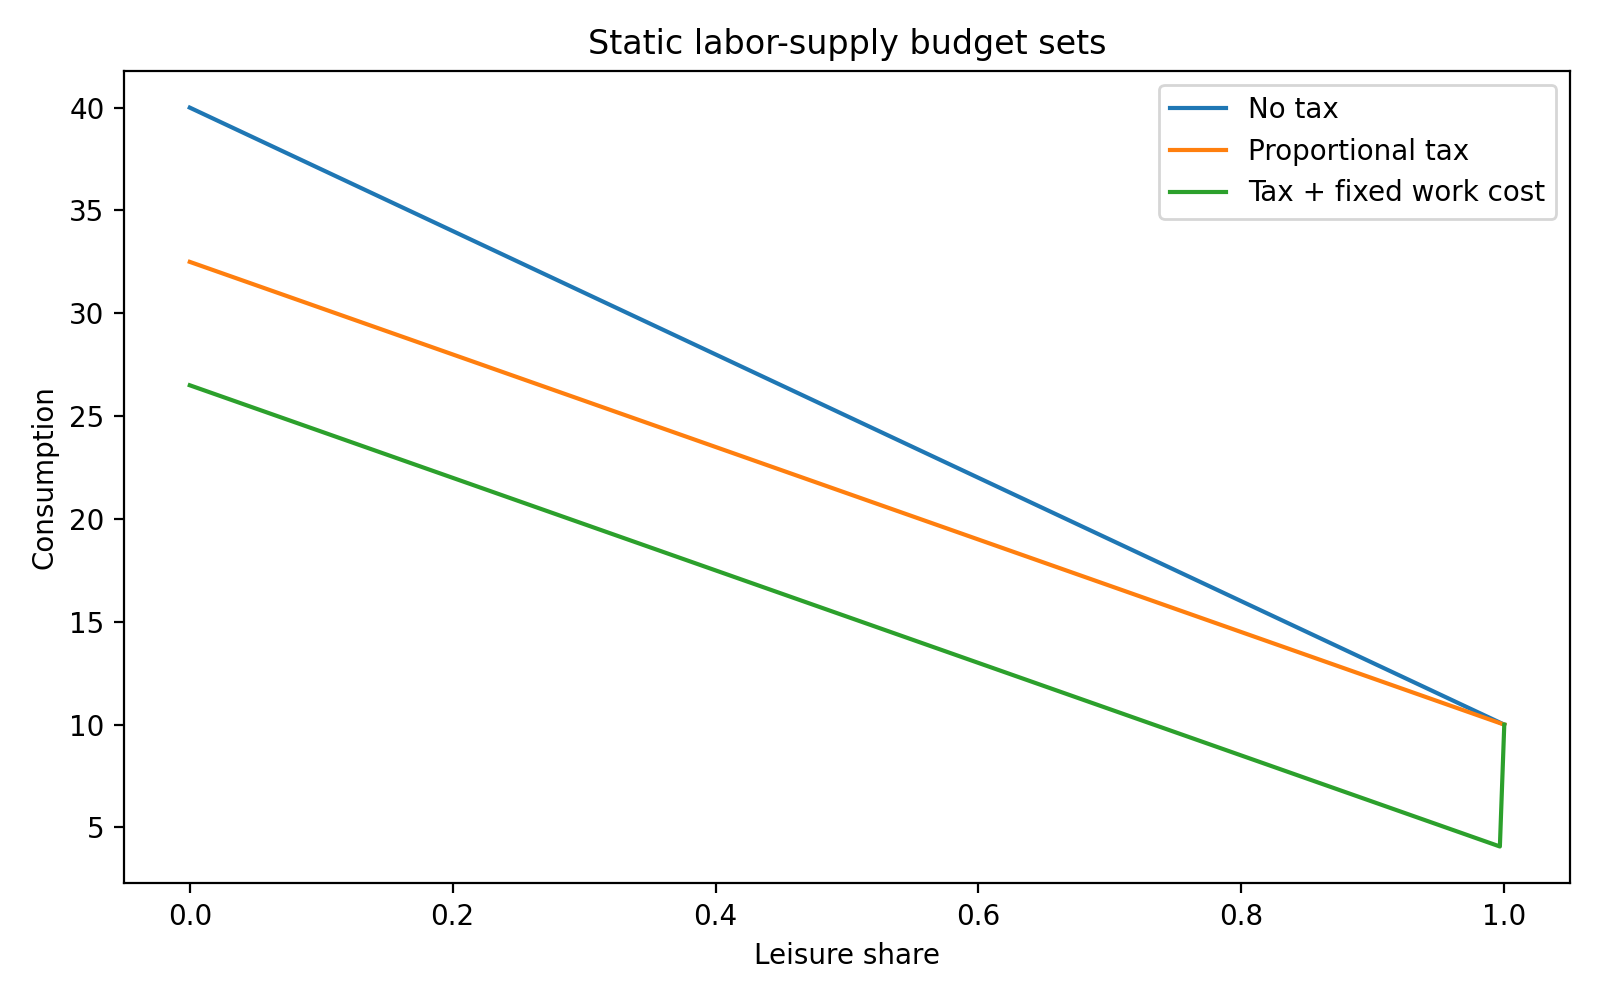
\includegraphics[width=0.88\linewidth]{02-static-budget-sets.png}
\end{center}
\end{frame}

\begin{frame}{Nonlinear schedules are the policy norm}
\begin{center}
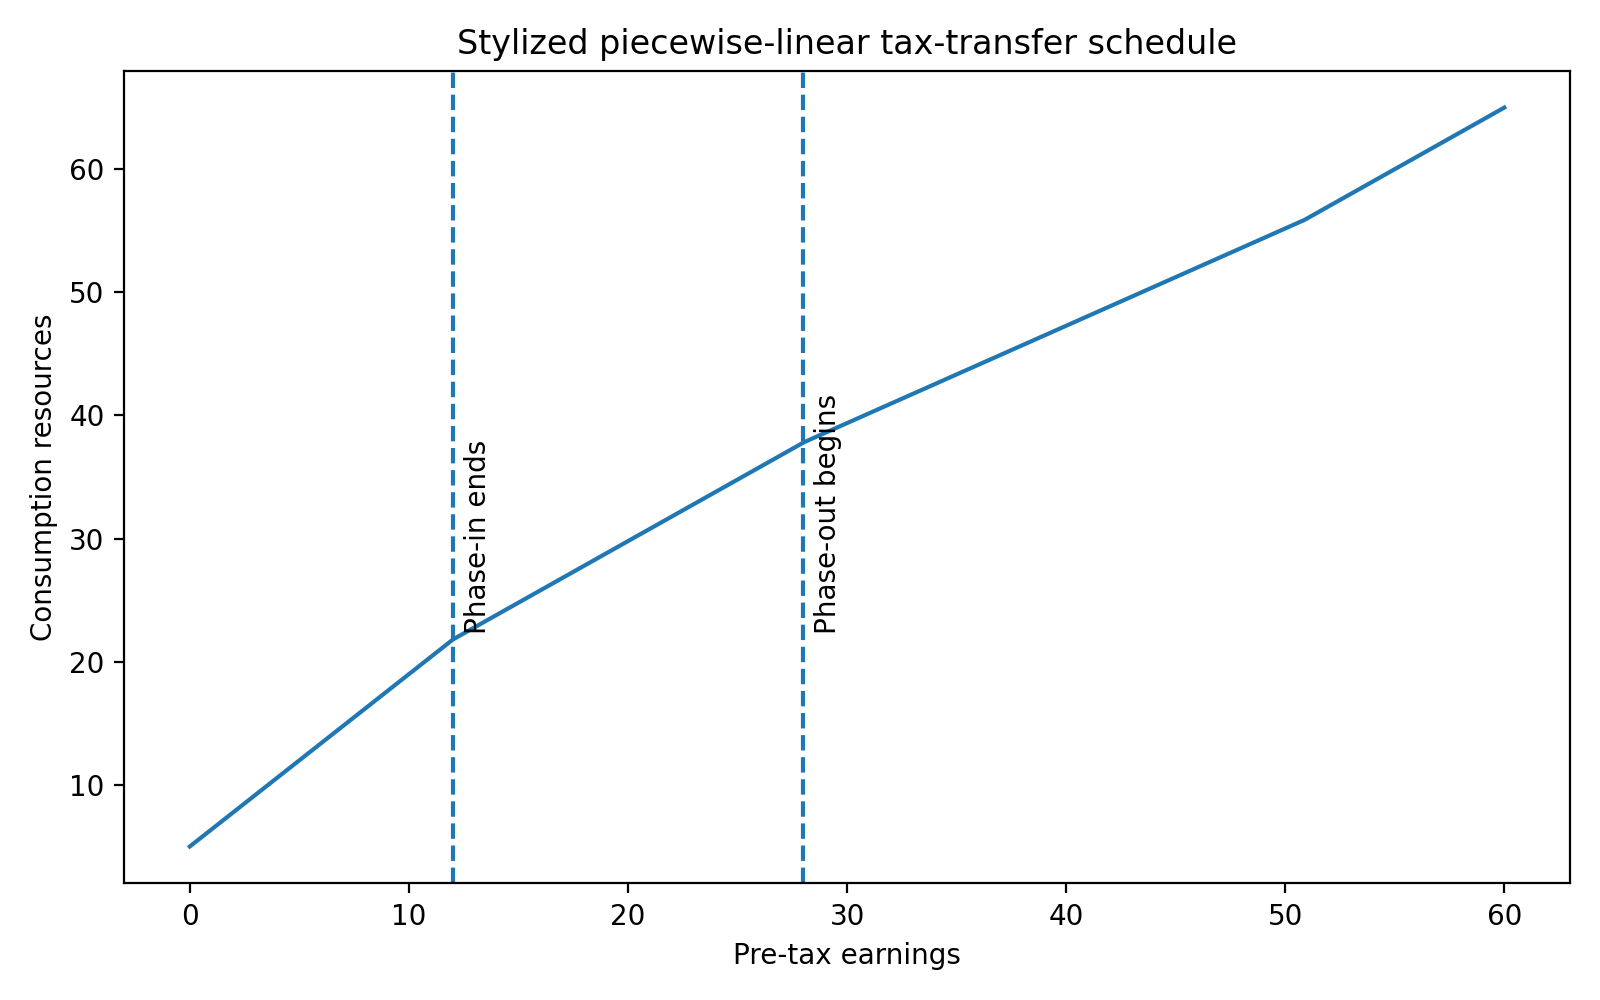
\includegraphics[width=0.88\linewidth]{02-eitc-schematic.png}
\end{center}
\end{frame}

\begin{frame}{Elasticity taxonomy}
\small
\begin{tabular}{p{0.27\linewidth} p{0.20\linewidth} p{0.40\linewidth}}
\toprule
Object & Margin & Main warning \\
\midrule
Uncompensated intensive elasticity & Hours & Mixes income and substitution effects \\
Compensated intensive elasticity & Hours & Needs stronger structure \\
Participation elasticity & Work / nonwork & Sensitive to fixed costs and benefit loss \\
Taxable-income elasticity & Earnings / reporting & May not be real labor supply \\
Macro elasticity & Aggregate hours & Includes equilibrium and institutions \\
\bottomrule
\end{tabular}
\end{frame}

\begin{frame}{Why the EITC is the applied bridge}
\begin{itemize}
    \item Phase-in region raises the payoff to entering work.
    \item Plateau and phase-out regions create different marginal incentives for current workers.
    \item The same policy can move single mothers, married couples, and secondary earners differently.
\end{itemize}
\end{frame}

\begin{frame}{Evidence map}
\begin{itemize}
    \item Eissa and Liebman: strong participation responses for single mothers.
    \item Eissa and Hoynes: married-couple responses depend on household earnings position.
    \item Saez: local bunching around kink points reveals responses to nonlinear schedules.
    \item Chetty, Friedman, and Saez: knowledge frictions shape observed EITC responses.
\end{itemize}
\end{frame}

\begin{frame}{What Week 2 feeds next}
\begin{itemize}
    \item Week 3: dynamic labor supply and lifecycle adjustment.
    \item Week 11: worker-side policy evaluation across taxes, transfers, childcare, and leave.
    \item Week 12: information, attention, and behavioral frictions in labor supply.
\end{itemize}
\end{frame}

\begin{frame}{Takeaways}
\begin{itemize}
    \item Static labor supply is the benchmark map from policy wedges to behavior.
    \item The key empirical question is often which margin is moving, not whether labor supply exists.
    \item Nonlinear schedules, fixed costs, and frictions make local interpretation essential.
    \item The EITC literature is the cleanest bridge from geometry to evidence.
\end{itemize}
\end{frame}

\end{document}
